\todo[inline]{The Position of the meniskus was exported with paraview in the decomposed state. The position was then extracted with a python script.Probe data was preprocessed as well and several computations for eval of simulations. Plots were generated with matplotlib?; Start of real results with an overview when what where. Maybe work with normalized data? }


Wie in Kapitel \ref{sec: capillaryRise} gezeigt, ist der Kapillare Aufstieg bis heute nicht verstanden. Ziel dieser Arbeit ist es daher 


Wie bereits beschrieben soll der Übergang vom linearen Anstieg der höhe einer Wassersäule in einer Kapillare hin zum Lucas Washburn Regime Untersucht werden. Weiter wurde beschrieben wie Delanoy et al. \cite{delannoy2019DualRoleViscosity} oder Ruiz et al. \cite{ruiz-gutierrez2022LongCrossoverDynamics} das Wachstum beschrieben. Zum Vergleich damit werden zunächst die Zeitpunkte oder Längen anhand ihrer vorhersagen berechnet und anschließend verglichen. Zunächst aber ein direkter Vergleich mit der Lucas-Washburn Gleichung. 
Delanoy et al. \cite{delannoy2019DualRoleViscosity} oder Ruiz et al. \cite{ruiz-gutierrez2022LongCrossoverDynamics} haben eigene Ansätze gefunden, um den Übergang zwischen den beiden Wachstumsregionen zu beschreiben. 


Im folgenden werden die Ergebnisse der Simulationen diskutiert und versucht eine Beschreibung für den Übergang der vorgestellten Wachstumsregionen des Kapillaren Aufstiegs zu finden. Um mögliche einflüsse durch den Kontaktwinkel berücksichtigen zu können wurden die Simulationen mit drei unterschiedlichen Kontaktwinkeln durchgeführt. Bei den verwendeten Dimensionen der Kapillare und der Flüssigkeiten, ist zu erwarten, dass der Einfluss der Gravitation vernachlässigbar ist, was auch in gesondert durchgeführten Simulationen gezeigt werden konnte, jedoch aufgrund der geringen aussagekraft eines Vergleichs mit Simulationen ohne Gravitation nicht weiter betrachtet wird. Damit wird jedoch auch klar, dass eine der besprochenen von Lucas und Washburn angenommen Vereinfachnungen für diesen Fall nicht gelten und eine Abweichung der vorhersage mit Gleichung \ref{eq: LW-Eq} darauf zurückzuführen ist, dass ein Gleichgewicht zwischen Kapillarkraft und viskosem drag nicht ausreicht, um den Kapillaren Aufstieg in frühen imbibitionsstadien zu beschreiben. 

Abbildung \ref{fig: LW-PFF_comp} zeigt einen direkten vergleich der Simulationsergebnisse mit der Lucas-Washburn Gleichung (rote linie \todo{describe as in actual figure later}). Darin wurde in \ref{fig: LW-PFF_comp} (a) linear skalliert und in \ref{fig: LW-PFF_comp} (b) logarithmisch. In der logarithmischen Darstellung werden die Unterschiede deutlich sichtbar. Zu Beginn ist die Steigung der Simulationen größer als die der vorhersage, bis sie sich schließlich annähern. Das lässt darauf schließen, dass der Kapillare Aufstieg erst nach einiger Zeit dem bekannten Lucas Washburn Wachstum folgt. Dies 

Wie ebenfalls bereits beschrieben sagt die Lucas-Washburn Gleichung ein Wachstum von $z(t)\sim \sqrt{t}$ vorher. 

\begin{figure}[h]
    \centering
    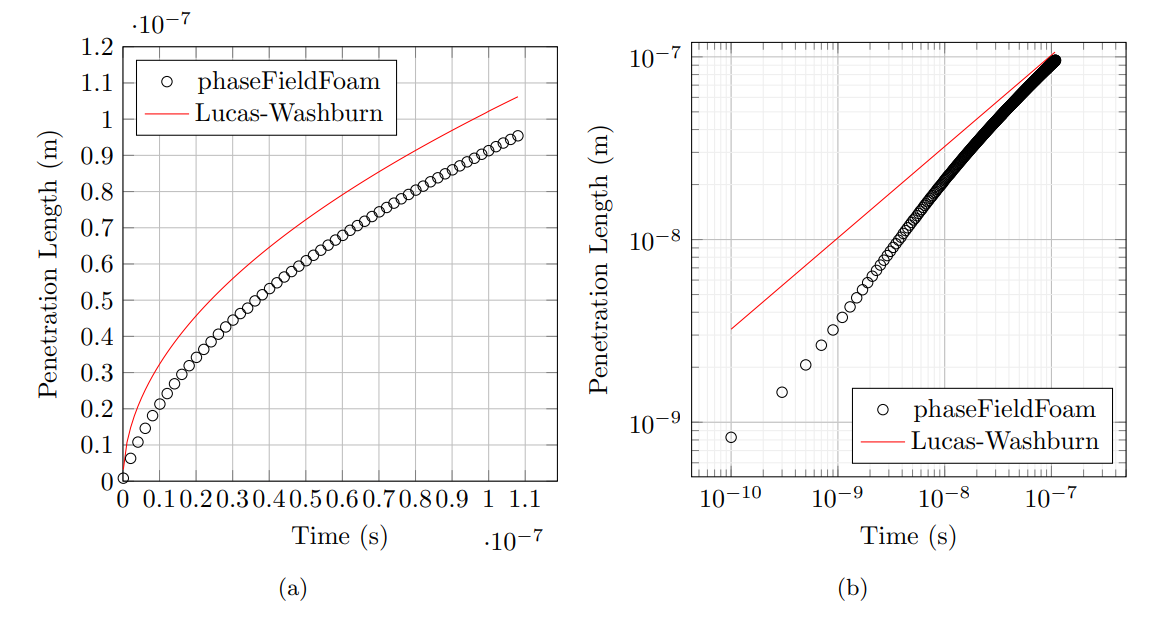
\includegraphics[width=.95\textwidth]{Pictures/LW-PFF_comp.png}
    \caption{Vergleich des von Lucas-Washburn vorhergesagten Wachstums mit den Ergenissen von \texttt{phaseFieldFoam}}
    \label{fig: LW-PFF_comp}
\end{figure}